\section{Alternating-Updating NMF Algorithms}
\label{sec:aunmf}

We define Alternating-Updating NMF algorithms as those that (1) alternate between updating $\WW$ for a given $\HH$ and updating $\HH$ for a given $\WW$ and (2) use the Gram matrix associated with the fixed factor matrix and the product of the input data matrix $\AA$ with the fixed factor matrix.
We show the structure of the framework in Algorithm \ref{alg:aunmf}. 

%Different algorithms determine $\WW$ and $\HH$ by partitioning these matrices in different ways and can be explained under Block Coordinate Descent (BCD) framework. 
%Generally, these matrices are determined as (a) 2-Blocks of entire matrix $\WW$ and $\HH$; (b) $2k$ blocks such as $[\ww^1, \ww^2, \cdots , \ww^m] \in \Rnplus{k}$ and $[\hh_1^T, \hh_2^T, \cdots , \hh_n^T] \in \Rnplus{k}$ \footnote{For convenience, $\M{x}^i$ is the $i$th column vector of matrix $\M{X}$ and $\M{x}_i$ is the $i$th row vector} and (c) $(m+n)k$ scalar blocks of $w_{ik} \in \WW$ and $h_{kj} \in \HH$. 

\begin{algorithm}
\caption{$[\WW,\HH] = \text{AU-NMF}(A,k)$}
\label{alg:aunmf}
\begin{algorithmic}[1]
\Require $\AA$ is an $m\times n$ matrix, $k$ is the approximation rank
\State Initialize $\HH$ with a non-negative matrix in $\Rn{n\times k}_+$.
\While{stopping criteria not satisfied} \label{algo:nmfloop}
  \State Update $\WW$ using $\HH \HH^T$ and $\AA \HH^T$
  %\State Update $\WW$ as $\Argmin{\tilde \WW\geq 0}\NormBr{\AA-\tilde\WW\HH}_F$
  %\State Update all blocks defined over $\WW$
  \label{line:aunmf:W}
  \State Update $\HH$ using $\WW^T\WW$ and $\WW^T \AA$
  %\State Update $\HH$ as $\Argmin{\tilde\HH\geq 0}\NormBr{\AA-\WW\tilde\HH}_F$
  %\State Update all blocks defined over $\HH$
  \label{line:aunmf:H}
\EndWhile
\end{algorithmic}
\end{algorithm}


The specifics of lines \ref{line:aunmf:W} and  \ref{line:aunmf:H} depend on the NMF algorithm, and we refer to the computation associated with these lines as the Local Update Computations (\LUC), as they will not affect the parallelization schemes we define in Section \ref{sec:parNMF}.
Because these computations are performed locally, we use a function $F(m,n,k)$ to denote the number of flops required for each algorithm's \LUC\ (and we do not consider communication costs).
Note that $F(m,n,k)$ does not include the cost of computing $\HH\HH^T$, $\WW^T\WW$, $\WW^T\AA$, or $\AA\HH^T$.

We note that AU-NMF is very similar to a two-block, block coordinate descent (BCD) framework, but it has a key difference.
In the BCD framework where the two blocks are
the unknown factors $\WW$ and $\HH$, 
we \emph{solve} the following subproblems,
which have a unique solution for a full rank $\HH$ and $\WW$: 
\SplitN{\label{eqn:two block}} {
\WW &\leftarrow \Argmin{\tilde \WW\geq 0}\NormBr{\AA-\tilde\WW\HH}_F,\\
\HH &\leftarrow  \Argmin{\tilde\HH\geq 0}\NormBr{\AA-\WW\tilde\HH}_F.
}
Since each subproblem involves nonnegative least squares,
this two-block BCD method is also called
the Alternating Non-negative Least Squares (ANLS) method \cite{kim2013nonnegative}.
For example, Block Principal Pivoting (\BPP), discussed more in detail at Section \ref{sec:BPP}, is 
one algorithm that solves these NLS subproblems.
In the context of the AU-NMF algorithm,
 an ANLS method {\em maximally} reduces 
the overall NMF objective function value 
by finding the optimal solution for
 given $\HH$ and $\WW$ in lines \ref{line:aunmf:W} 
and \ref{line:aunmf:H} respectively.  

There are other popular NMF algorithms 
that update the factor matrices alternatively
without maximally reducing the objective function value each time,
in the same sense as in ANLS. 
These updates do not necessarily solve each of the subproblems \eqref{eqn:two block} to optimality but simply improve the overall objective function \eqref{eqn:original NMF}.  
Such methods include Multiplicative Update (\MU) \cite{seung2001algorithms} and Hierarchical Alternating Least Squares (\HALS) \cite{cichocki2009nonnegative}, which was also proposed as Rank-one Residual Iteration (RRI) \cite{Ho2008}.
To show how these methods can fit into the AU-NMF framework, we discuss them in more detail in Sections \ref{sec:MU} and \ref{sec:HALS}.

The convergence properties of these different algorithms are discussed in detail by Kim, He and Park \cite{kim2013nonnegative}. 
We emphasize here that both \MU\ and \HALS\ require computing Gram matrices and matrix products of the input matrix and each factor matrix.
Therefore, if the update ordering follows the convention of updating all of $\WW$ followed by all of $\HH$, both methods fit into the AU-NMF framework. 
We note that both \MU\ and \HALS\ are defined for more general update orders, but for our purposes we constrain them to be AU-NMF algorithms.

While we focus on three NMF algorithms in this paper, we highlight that our framework is extensible to other NMF algorithms, including those based on Alternating Direction Method of Multipliers (ADMM) \cite{SF14}, Nesterov-based methods \cite{GTLY12}, or any other method that fits the framework of Algorithm \ref{alg:aunmf}.

%Here, we have explained the update equations of the NMF algorithms ANLS/BPP, HALS and MU. In all these three algorithms, the update equations uses $\AA\HH^T$ and $\HH\HH^T$ for line \ref{line:anls:W} and $\WW^T\AA$ and $\WW^T\WW$ for line \ref{line:anls:H}.

%As in the Figure \ref{fig:2blocks}, the ANLS/BPP \cite{kim2011fast} is an example of 2-Blocks BCD that determines $\WW$ and $\HH$ as matrix blocks by solving 
%the following equations using active set method iteratively until a stopping criteria is satisfied: 


%\begin{figure*}
%\subfloat[][ANLS/BPP 2-Blocks BCD] {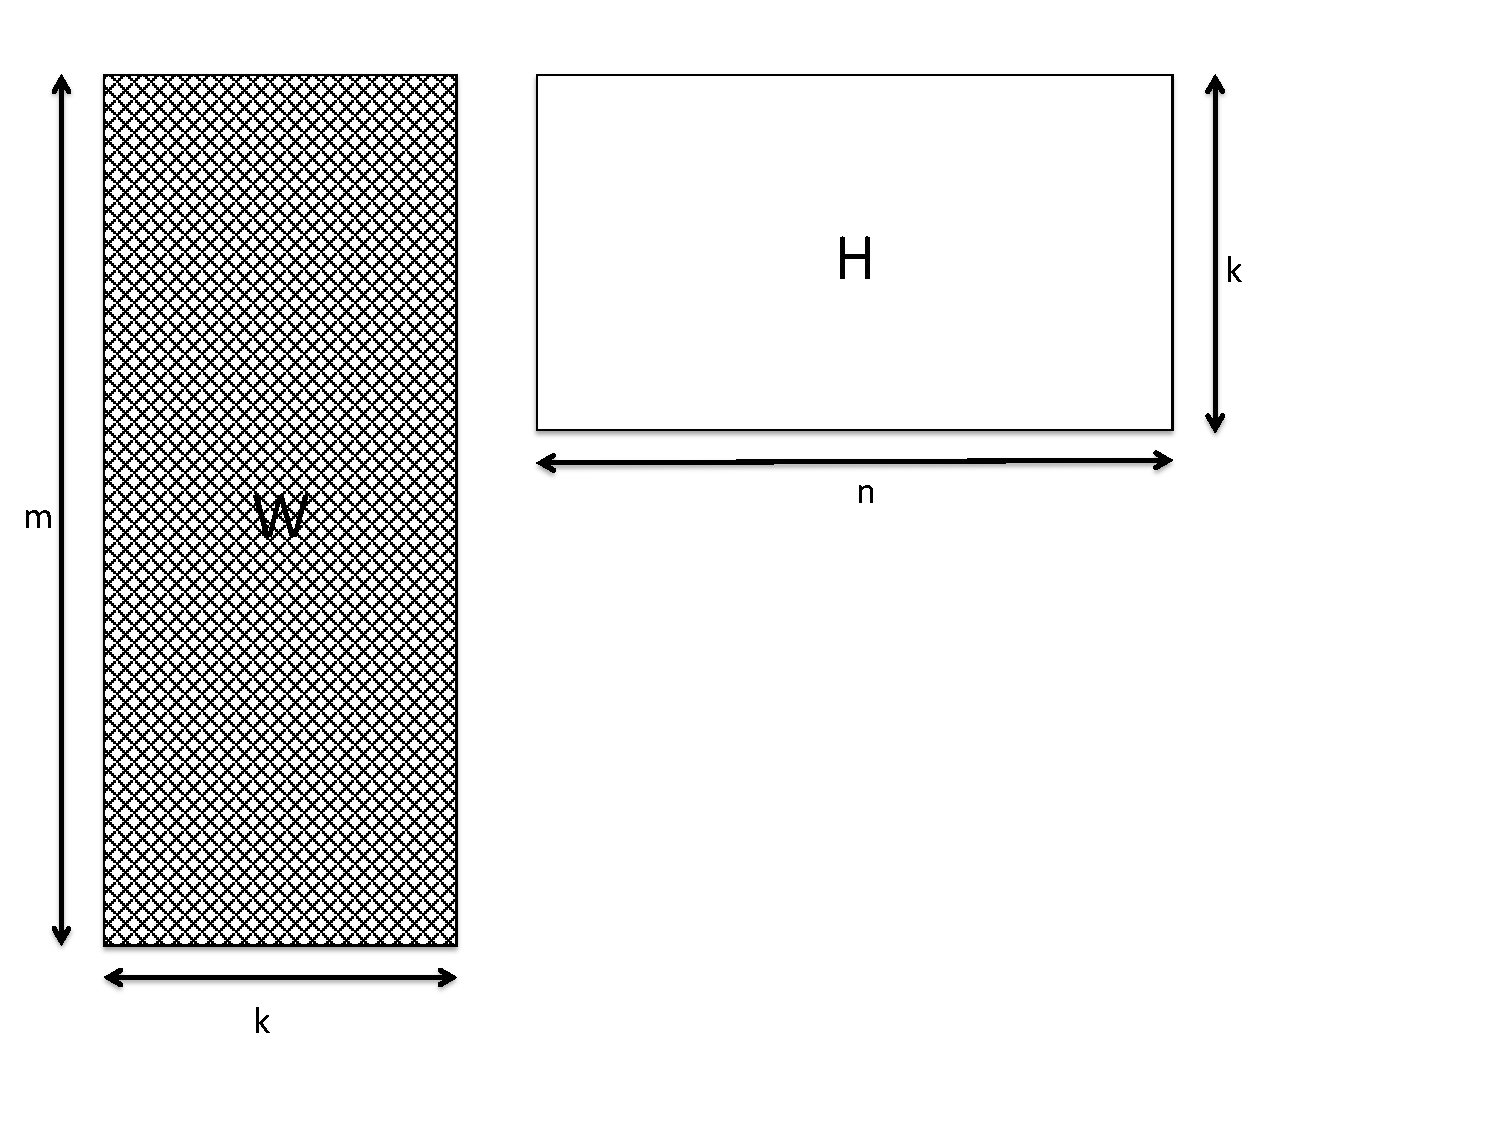
\includegraphics[height=1.5in, width=2.5in]{fig/bcd2blocks}\label{fig:2blocks}}
%\subfloat[][HALS 2k-Blocks BCD] {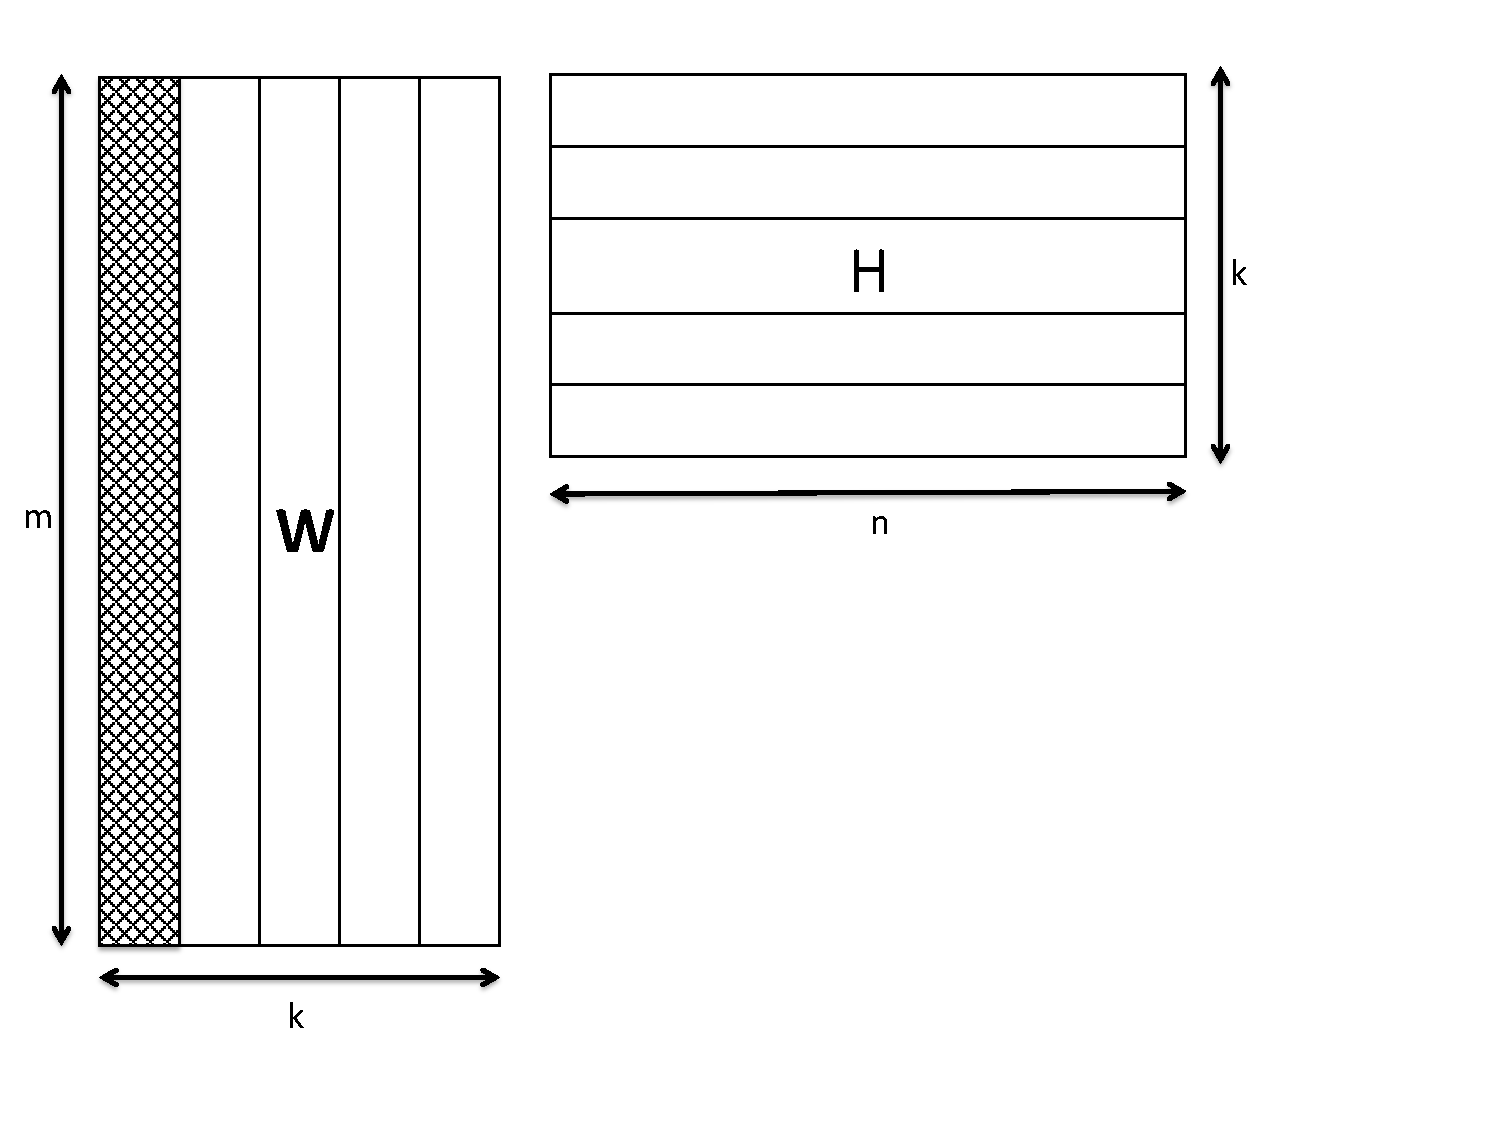
\includegraphics[height=1.5in, width=2.5in]{fig/bcd2kblocks}\label{fig:2kblocks}}
%\subfloat[][MU (m+n)k Scalar Blocks BCD] {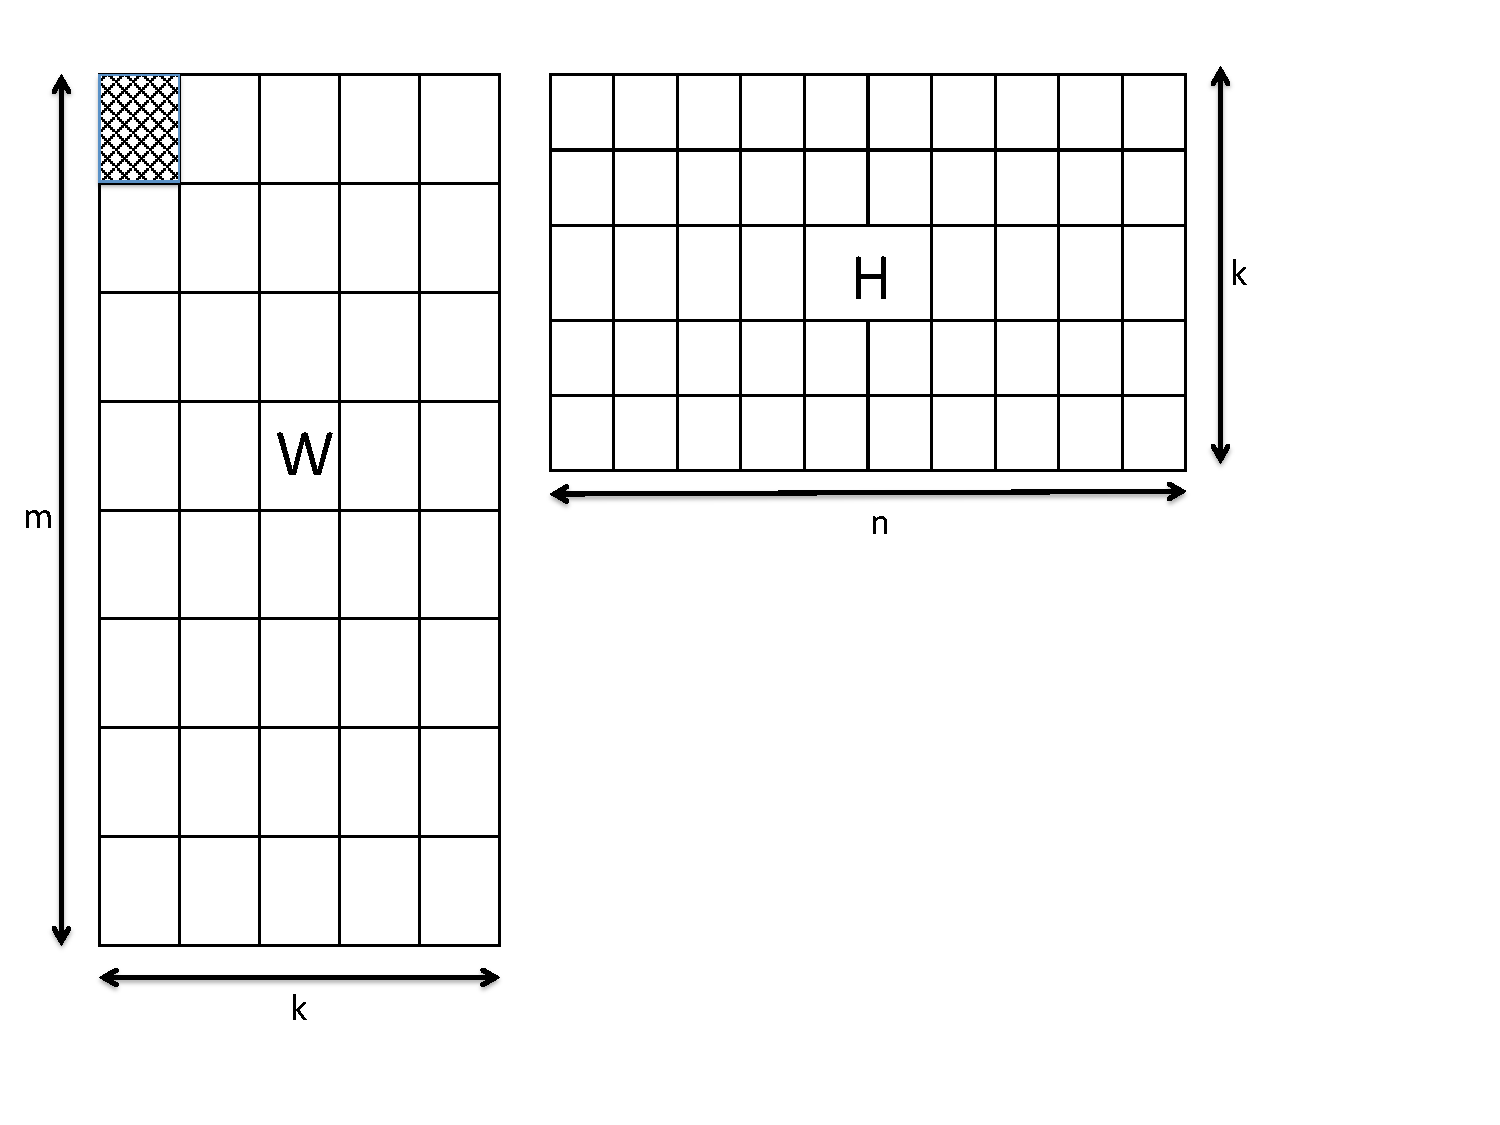
\includegraphics[height=1.5in, width=2.5in]{fig/bcdscalarblocks}\label{fig:bcdscalarblocks}}
%\end{figure*}

\subsection{Multiplicative Update (\MU)}
\label{sec:MU}

In the case of \MU\ \cite{seung2001algorithms}, individual entries of $\WW$ and $\HH$ are updated with all other entries fixed.
In this case, the update rules are 
\SplitN{\label{eqn:muupdate}} {
w_{ij} &\leftarrow w_{ij} \frac{(\AA \HH^T)_{ij}}{(\WW \HH \HH^T)_{ij}}, \text{ and }\\
h_{ij} &\leftarrow  h_{ij} \frac{(\WW^T \AA)_{ij}}{(\WW^T \WW \HH)_{ij}}.
} 
Instead of performing these $(m+n)k$ in an arbitrary order, if all of $\WW$ is updated before $\HH$ (or vice-versa), this method also follows the AU-NMF framework.
After computing the Gram matrices $\HH\HH^T$ and $\WW^T \WW$ and the products $\AA\HH^T$ and $\WW^T\AA$, the extra cost of computing $\WW (\HH\HH^T)$ and $(\WW^T\WW)\HH$ is $F(m,n,k)=2(m+n)k^2$ flops to perform updates for all entries of $\WW$ and $\HH$, as the other elementwise operations affect only lower-order terms.
Thus, when \MU\ is used, lines \ref{line:aunmf:W} and \ref{line:aunmf:H} in Algorithm \ref{alg:aunmf} -- and functions UpdateW and UpdateH in Algorithms \ref{alg:naive} and \ref{alg:2D} -- implement the expressions in \eqref{eqn:muupdate}, given the previously computed matrices.  


\subsection{Hierarchical Alternating Least Squares (\HALS)}
\label{sec:HALS}

In the case of \HALS\ \cite{cichocki2009nonnegative,CA2009}, updates are performed on individual columns of $\WW$ and rows of $\HH$ with all other entries in the factor matrices fixed.
This approach is a BCD method with $2k$ blocks, set to minimize the function
\begin{equation}
f(\ww^1,\cdots,\ww^k,\hh_1,\cdots,\hh_k)=\lt\|\AA-\sum_{i=1}^k \ww^i \hh_i \rt\|_F,\label{eq:hals_obj}
\end{equation}
where $\ww^i$ is the $i$th column of $\WW$ and $\hh_i$ is the $i$th row of $\HH$.
The update rules \cite[Algorithm 2]{CA2009} can be written in closed form:
\SplitN{\label{eqn:halsupdate}} {
\ww^i &\leftarrow \lt[ \ww^i + (\AA\HH^T)^i - \WW (\HH \HH^T)^i \rt]_+ \\
\ww^i &\leftarrow \frac{\ww^i}{\|\ww^i\|}, \text{ and } \\
\hh_i &\leftarrow \lt[ \hh_i + (\WW^T\AA)_i - (\WW^T \WW)_i\HH \rt]_+.
} 

%\grey{We need to explain this normalization, citing a HALS paper or something similar.}
Note that the columns of $\WW$ and rows of $\HH$ are updated in order, so that the most up-to-date values are always used, and these $2k$ updates can be done in an arbitrary order.  However, if all the $\WW$ updates are done before $\HH$ (or vice-versa),  the method falls into the AU-NMF framework.
After computing the matrices $\HH\HH^T$, $\AA\HH^T$, $\WW^T\WW$, and $\WW^T\AA$, the extra computation is $F(m,n,k)=2(m+n)k^2$ flops for updating both $\WW$ and $\HH$. 

Thus, when \HALS\ is used, lines \ref{line:aunmf:W} and \ref{line:aunmf:H} in Algorithm \ref{alg:aunmf} -- and functions UpdateW and UpdateH in Algorithms \ref{alg:naive} and \ref{alg:2D} -- implement the expressions in \eqref{eqn:halsupdate}, given the previously computed matrices.  

%Note that the normalization of columns of $\WW$ is unique to $\; this does introduce extra 
%In practice, we also found without such normalization, the error was oscillating and it promised the monotonic error reduction to \HALS\ algorithm.

%According to \cite{kim2013nonnegative}, the above update function of MU does not find the optimal blocks $w_{ij}$ and discuss a different optimal update for scalar blocks function that is similar to HALS. 



%In general, many of the NMF algorithms can be explained using the BCD framework. However, specifically it can be observed in all the above three different cases of NMF algorithms explained above, the blocks of the matrix $\WW$ is updated first followed by the updates to matrix $\HH$ and we always use the most recent blocks of $\WW$ and $\HH$ matrix. In this paper, we define iteration as one pass of updating all the blocks of low rank factors $\WW$ and $\HH$. That is., in the case of 2-Blocks, updating entire $\WW$, $\HH$; for $2k$-blocks finding all the vectors of $\WW$, $\HH$; and all the elements of $\WW$, $\HH$ for scalar blocks BCD. 

\subsection{Alternating Nonnegative Least Squares with Block Principal Pivoting}
\label{sec:BPP}

%In this paper, we focus on and use the BPP method \cite{kim2011fast} to solve the NLS problem, as it is the fastest algorithm (in terms of number of iterations). 
%As argued in Section \ref{sec:aunmf}, we note that many NMF algorithms, including MU and HALS, can be used within our parallel frameworks (Algorithms \ref{alg:naive} and \ref{alg:2D}).  

Block Principal Pivoting (BPP) is an active-set-like method for solving the NLS subproblems in Eq. \eqref{eqn:two block}.
The main subroutine of BPP is the single right-hand side NLS problem
\SplitN{\label{eqn:single NLS}}{
\min_{\xx\geq 0} \|\CC\xx-\mathbf{b}\|_2.
}

The Karush-Kuhn-Tucker (KKT) optimality conditions for  Eq.~\eqref{eqn:single NLS} are as follows
\SplitS{\label{eqn:KKT}}{
\yy &= \CC^T \CC \xx - \CC^T \mathbf{b} \\
\xx,\yy &\geq 0\\
%\xx &\geq 0\\
x_i y_i & = 0 \;\; \forall i .
}
The KKT conditions \eqref{eqn:KKT} states that at optimality, the support sets (i.e., the non-zero elements)
of $\xx$ and $\yy$ are complementary to each other. Therefore, Eq.~\eqref{eqn:KKT} is an instance of
the \emph{Linear Complementarity Problem} (LCP) which arises frequently in quadratic programming.
When $k\ll\min(m,n)$, active-set and active-set-like methods are very suitable because most
computations involve matrices of sizes $m\times k, n\times k$, and $k\times k$ which are
small and easy to handle.

If we knew which indices correspond to nonzero values in the optimal solution, then computing the solution is an unconstrained least squares problem on these indices.
In the optimal solution, call the set of indices $i$ such that $x_i=0$ the active set, and let the remaining indices be the passive set. The BPP algorithm works to find this final active set and passive set. 
%Since the above problem is convex, the correct partition of the optimal solution will satisfy the KKT condition (Eq.~\eqref{eqn:KKT}).  
It greedily swaps indices between the intermediate active and passive sets until finding a partition that satisfies the KKT condition. In the partition of the optimal solution, the values of the indices that belong to the active set will take zero. The values of the indices that belong to the passive set are determined by solving the unconstrained least squares problem restricted to the passive set. Kim, He and Park \cite{kim2011fast}, discuss the BPP algorithm in further detail. 
We use the notation
$$\XX \gets \text{SolveBPP}(\CC^T\CC,\CC^T\BB)$$
to define the (local) function for using BPP to solve Eq.~\eqref{eqn:single NLS} for every column of $\XX$.
We define $C_\text{BPP}(k,c)$ as the cost of \text{SolveBPP}, given the $k\times k$ matrix $\CC^T\CC$ and $k\times c$ matrix $\CC^T\BB$. 
\text{SolveBPP} mainly involves solving least squares problems over the intermediate passive sets. 
%and has a worst case of solving $k$ least squares problems. 
Our implementation uses the normal equations to solve the unconstrained least squares problems because the normal equations matrices have been pre-computed in order to check the KKT condition.
However, more numerically stable methods such as QR decomposition can also be used.

Thus, when \BPP\ is used, lines \ref{line:aunmf:W} and \ref{line:aunmf:H} in Algorithm \ref{alg:aunmf} -- and functions UpdateW and UpdateH in Algorithms \ref{alg:naive} and \ref{alg:2D} -- correspond to calls to SolveBPP.
The number of flops involved in SolveBPP is not a closed form expression; in this case $F(m,n,k)=C_\text{BPP}(k,m)+ C_\text{BPP}(k,n)$.

